\subsection{E--I plasticity moves single-neuron responses toward higher efficiency, with lifetime CV acting as a limited proxy}
\label{sec:single_neuron_ice}

The Gibbs manifold is defined by the optimization problem and is independent of circuit implementation; biological mechanisms regulate the operating point along it rather than reshaping its geometry.  We test whether inhibitory STDP combined with E--I balance is sufficient to drive an individual neuron in the direction predicted by the framework, and we use this model to expose the limits of $\mathrm{CV}_L$ as a proxy for the distributional CV.

We simulated a conductance-based neuron receiving eight input pathways under inhibitory STDP \cite{16,sp_stdp} (Fig.~\ref{fig:single-neuron}A; Methods).  As E--I balance tightens, the mean currents stabilize and the $I_\mathrm{EX}/I_\mathrm{IN}$ ratio approaches unity (Fig.~\ref{fig:single-neuron}B), while instantaneous traces shift from dense overlapping inputs to sparse, punctuated events with progressively sharper stimulus selectivity (Fig.~\ref{fig:single-neuron}C--D).  Stimulus separability $\bar{U}$ (mean off-diagonal of the pairwise cosine-similarity matrix between per-channel current profiles) rises monotonically from $0.61$ to $0.95$ across learning (Fig.~\ref{fig:single-neuron}D).

ICE and $\mathrm{CV}_L$ co-increase during the early phase of learning (Fig.~\ref{fig:single-neuron}E), consistent with the predicted ICE--CV monotonicity.  As E--I balance tightens further, however, the two decouple: $\mathrm{CV}_L$ peaks and then declines while ICE keeps rising.  This decoupling exposes a generic limitation of $\mathrm{CV}_L$ as an empirical proxy: refractory period and membrane time constant impose a hard ceiling on attainable ISI distributions.  Once this ceiling is reached, further ICE gains come from mechanisms that $\mathrm{CV}_L$ cannot capture---sharpened stimulus selectivity redistributes activity across the response space, increasing the spread of $p(r)$ without increasing the temporal irregularity of individual spike trains.  Plotted against the E--I current ratio (Fig.~\ref{fig:single-neuron}F), both ICE and $\mathrm{CV}_L$ follow exponential saturation with $I_\mathrm{EX}/I_\mathrm{IN}$, but $\mathrm{CV}_L$ saturates at a lower $I_\mathrm{EX}/I_\mathrm{IN}$ than ICE.

In the ICE--$\mathrm{CV}_L$ plane (Fig.~\ref{fig:single-neuron}G), the temporal trajectory rises rightward early, then folds back leftward while ICE continues upward; at late learning stages it exceeds the Gaussian-channel reference ($\sigma_n^2=10$; Methods), indicating that efficiency gains are driven by mechanisms beyond single-neuron temporal variability.  This motivates the more direct geometric test of the next section, where all three systems are projected onto the $I$--$C$ plane without relying on any single empirical CV proxy.

\begin{figure}[!h]
\centering
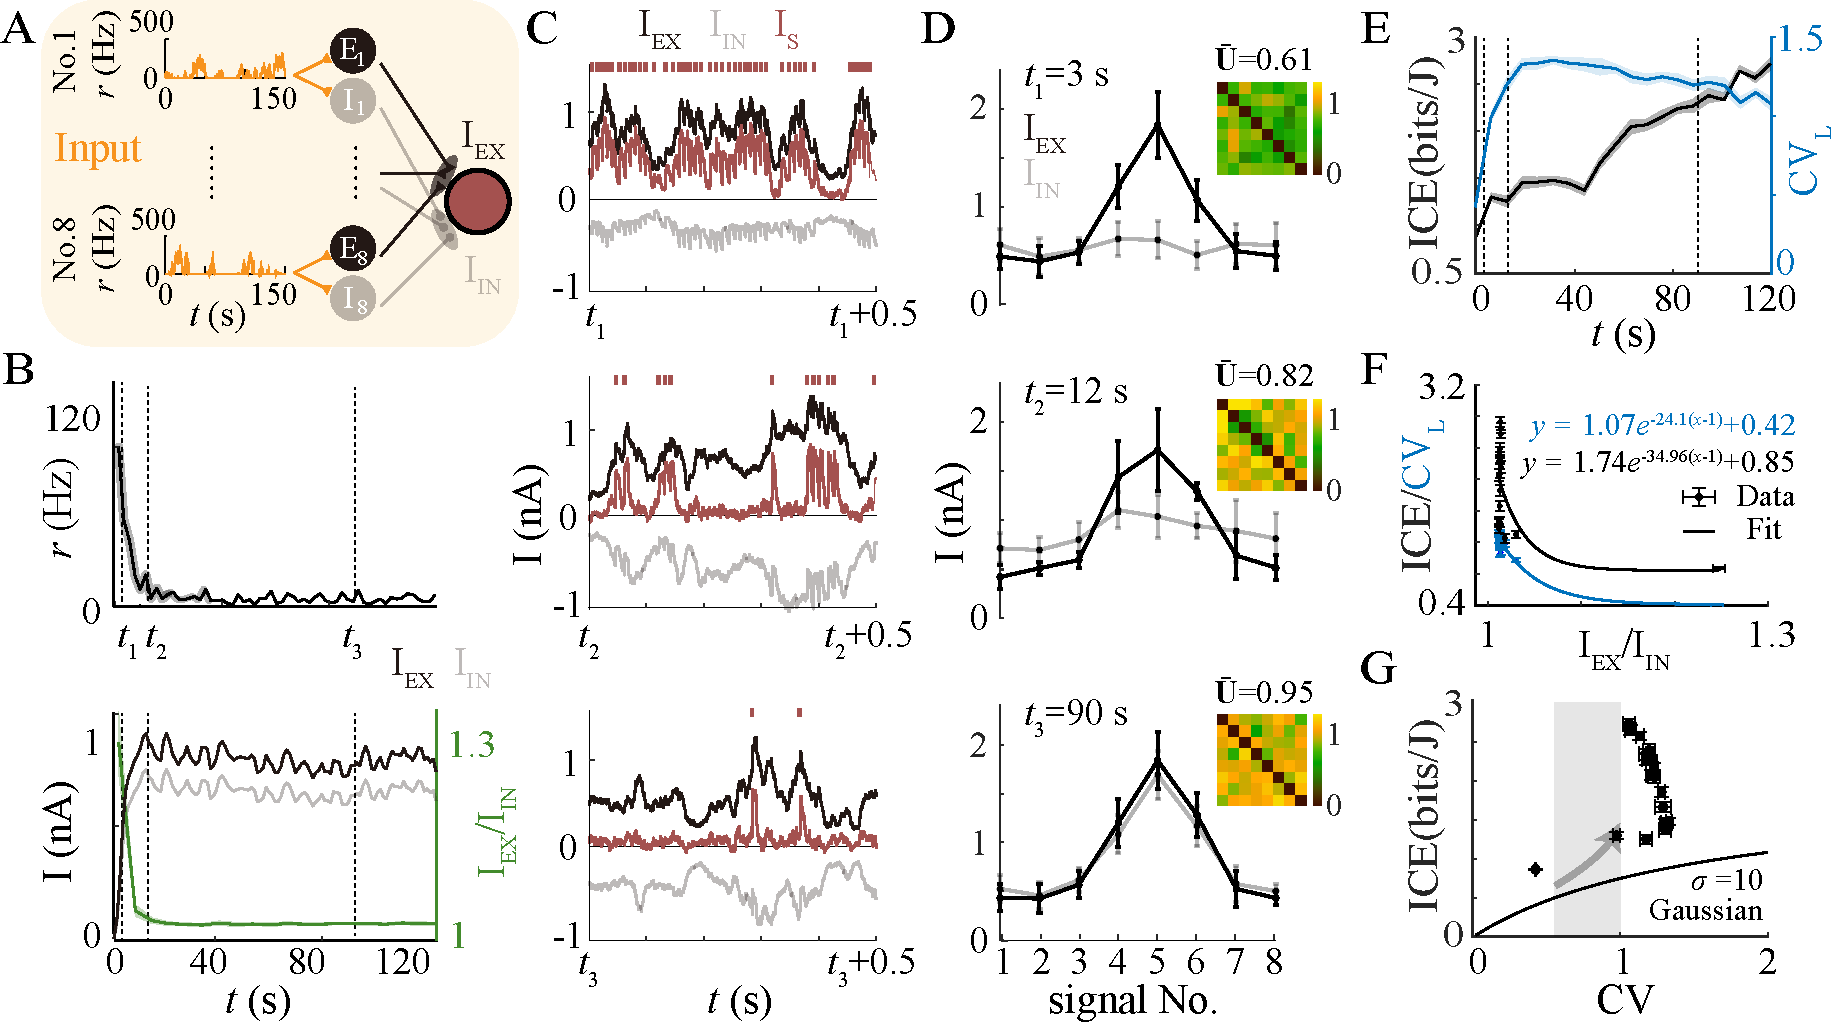
\includegraphics[scale=0.42]{figures/Figure3.pdf}
\caption{\textbf{Synaptic plasticity drives the neuron towards the Gibbs manifold of metabolically efficient codes.}
(\textbf{A}) Schematic: target neuron with 8 input channels, each with excitatory ($E_i$) and inhibitory ($I_i$) populations.
(\textbf{B}) Firing rate $r$ (top); mean $I_\mathrm{EX}$ (black) and $I_\mathrm{IN}$ (gray) currents with their ratio $I_\mathrm{EX}/I_\mathrm{IN}$ (green, right axis, baseline at 1) (bottom) over learning; dashed lines: $t_1, t_2, t_3$.
(\textbf{C}) Instantaneous current traces at $t_1, t_2, t_3$ ($I_\mathrm{EX}$ black, $I_\mathrm{IN}$ gray, stimulus $I_S$ red; red ticks: spikes).
(\textbf{D}) Per-channel current profiles and stimulus-separability matrix $\bar{U}$ at the three time points; $\bar{U}$ rises from $0.61$ to $0.95$.
(\textbf{E}) ICE (black, bits/J) and $\mathrm{CV}_L$ (blue) over time; $\mathrm{CV}_L$ peaks then declines after hitting its biophysical ceiling while ICE keeps rising.
(\textbf{F}) ICE and $\mathrm{CV}_L$ vs.\ $I_\mathrm{EX}/I_\mathrm{IN}$ with exponential fits ($y=ae^{-b(x-1)}+c$); $\mathrm{CV}_L$ saturates earlier and at a lower asymptote than ICE.
(\textbf{G}) ICE--$\mathrm{CV}_L$ plane: the temporal trajectory (grey arrow) rises in $\mathrm{CV}_L$ early and folds back leftward late while ICE keeps climbing, exposing the limits of $\mathrm{CV}_L$ as a proxy for distributional CV.  Data exceed the Gaussian channel reference ($\sigma_n^2 = 10$, black curve) at late training, indicating efficiency gains beyond single-neuron temporal variability; the grey shaded band marks the linear-cost CV range $[1/\sqrt{3},\,1]$ within which the Gibbs-optimal ICE--CV ceiling (Fig.~\ref{fig:figure1_conceptual_framework}C\textit{iii}, Supp.~Sect.~1.5) lies.}
\label{fig:single-neuron}
\end{figure}
